\documentclass[paper=a4, fontsize=12pt]{scrartcl}
\usepackage{graphicx}
\usepackage[protrusion=true,expansion=true]{microtype}
\usepackage{amsmath,amsfonts,amsthm}
\usepackage{fourier}
\usepackage[utf8]{inputenc}
\usepackage{amsmath}
\usepackage{amsfonts}
\usepackage{amssymb}
\usepackage[OT4]{fontenc}
\usepackage[polish]{babel}
\usepackage{epstopdf}
\usepackage{fancyhdr}
\usepackage{hyperref}
\pagestyle{fancyplain}
\fancyhead{}	
\renewcommand{\headrulewidth}{1pt}
\renewcommand{\footrulewidth}{1pt}
\textheight = 700pt
\textwidth = 500pt
\hoffset =-30pt
\begin{document}
\begin{flushright}
24.03.2016 r.\\
dr Robert Bryl
\end{flushright}Paweł Grabiński\\
Rok 3, Fizyka teoretyczna\\[0.5cm]
{\huge \bf Promieniowanie rentgenowskie}
\section{Wyniki}
\subsection{Stala Plancka}
Wartość stałej Plancka: $h=(6.65\pm0.049)\cdot10^{-34}\:\mathrm{J\cdot s}$.
\subsection{Stała sieci krystalicznej NaCl}
Wartość stałej sieci krystalicznej kryształu NaCl: $d=(5.52\pm0.04)\:\mathrm{\AA}$
\section{Opis teoretyczny}
\subsection{Promieniowanie rentgenowskie}

Promieniowanie elektromagnetyczne o fali z zakresu:
\begin{itemize}
	\item miękkie $\lambda=0.1-10\:\mathrm{nm}=10^{-10}-10^{-8}\:\mathrm{m}$
	\item twarde $\lambda=5-100\:\mathrm{pm}=5\cdot10^{-12}-10^{-10}\:\mathrm{m}$
\end{itemize}

Zródłem promieniowania rentgenowskiego są elektrony wyhamowywane na atomach tarczy w lampie rentgenowskiej.

Jednak akutalnie pojęcie promieniowania rentgenowskiego używa się, by nazywać promieniowanie z danego zakresu długości fali. Akutalnie buduje się lasery oraz synchrotrony służące do generowania promieniowania rentgenowskiego o długości fali znacznie krótszej niż w przypadku lampy rentgenowskiej.

Promieniowanie rentgenowskie ma zastosowanie w badaniach ciała stałego, medycynie (zdjęcia rentgenowskie) i w astronomii.
\begin{figure}
\centering
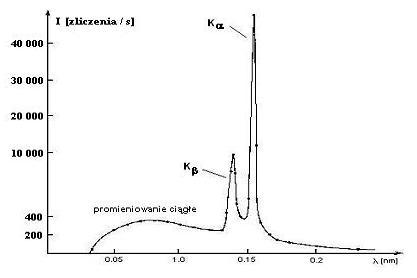
\includegraphics[width=0.7\linewidth]{promren}
\caption{Wykres natężenia promieniowania rentgenowskiego w zależności od długości fali. Widzimy część promieniowania ciągłego oraz dwa maksima odpowiadające promieniowaniu charakterystycznemu.}
\label{fig:promren}
\end{figure}

\subsubsection{Promieniowanie hamowania(ciągłe)}
Promieniowanie wytwarzanie w procesie rozpraszania wiązki elektornów na chmurze elektronowej atomów. Wykazuje dwie cechy charakterystyczne:
\begin{itemize}
	\item Krótkofalowa granica promieniowania - najmniejsza długość fali jaka może być wyprodukowana w tym procesie. Odpowiada sytuacji, gdy elektron całą swoją energię kinetyczną oddaje w postaci promieniowania:
	\begin{align*}
	eU=\frac{hc}{\lambda_{gr}} \qquad\Rightarrow\qquad \lambda_{gr}=\frac{hc}{eU}
	\end{align*}
	Natężenie wraz ze zbliżaniem się prawostronnym do tej wartości maleje do zera.
	\item Maksimum natężenia - tak jak cały wykres zależy od sprawności procesu. Sprawność jest proporcjonalna do liczby porządkowej pierwiastka z jakiego zbudowana jest tarcza(antykatoda).
\end{itemize}

\subsubsection{Poziomy energetyczne atomu}

Jak przewidział Bohr w swoim modelu atomu oraz jak wykazali Franck i Hertz w swoim doświadczeniu, atomy mają poziomy energetyczne. Są one związane z dyskretnymi energiami jakie mogą mieć elektrony w stanach związanych z jądrem atomu. Są one numerowane odpowiednimi liczbami kwantowymi. Elektron przechodząc pomiędzy różnymi stanami musi wymienić energię z otoczeniem w postaci fotonu o energi odpowiadającej różnicy stanów.
\subsubsection{Promieniowanie charakterystyczne}
Związane jest z wybijaniem elektronów z powłok, którym odpowiadają małe kwantowe liczby porządkowe. Elektron przeskakuje do pierwszego wolnego stanu. Atom w tym stanie jest niestabilny. Elektron powraca do stanu początkowego emitując kwant promieniowania o dużej energii. Alternatywnie może dojść do przejść kaskadowych, gdzie elektrony z pośrednich powłok będą przechodzić do niższych stanów, emitując fotony o różnych energiach.

\subsection{Stała Plancka}
Stała jaką wprowadził Max Planck w 1900 roku w swoim formaliźmie związany z emisją dyskretnych wartości energii promieniowania ciała doskonale czarnego. Energia emitowanego fotonu jest równa iloczynowi stałej Plancka oraz częstotliwości fali: \begin{align*}
E=h\nu.
\end{align*}
Stała Plancka zgodnie z aktualnym stanem wiedzy wynosi:
\begin{align*} 
h=6.626070040(81)\:\mathrm{J\cdot s}= 4.135667662(25)\:\mathrm{eV}
\end{align*}
Często używa się zredukowanej stałej Plancka: $\hbar=\frac{h}{2\pi}$.

\subsection{Struktura krystalograficzna}
Struktura opisująca uporządkowaną(wykazującą symetrie) budowę kryształów.\\
Na strukturę krystaliczną składają się:
\begin{itemize}
	\item sieć krystaliczna - abstrakcyjny zbiór węzłów(punktów) w przestrzeni rozpięty na trzech elementarnych wektorach translacji, niezależnie od przesunięcia o wektor będący całkowitą kombinacją liniową elementarnych wektorów translacji, sieć wygląda tak samo,
	\item baza atomowa - zbiór atomów odpowiadający jednemu węzłowi sieci, przemieszczając bazę można zbudować cały kryształ.
\end{itemize}
Po nałożeniu bazy atomowej na sieć krystaliczną otrzymujemy strukturę krystaliczną - fizyczny opis budowy kryształu.\\
Przykładem sieci krystalicznej może być układ \textit{fcc(ang. face centered cube)}. Zbudowany jest on na wektorach:
\begin{align*}
\vec{a}_1=\frac{d}{2}(\hat{x}+\hat{y})\qquad\vec{a}_2=\frac{d}{2}(\hat{y}+\hat{z})\qquad\vec{a}_3=\frac{d}{2}(\hat{z}+\hat{x})
\end{align*}
\subsubsection{Wskaźniki Millera}
Notacja używająca trzech liczb całkowitych do opisu płaszczyzn w krysztale.
\begin{figure}[h]
\centering
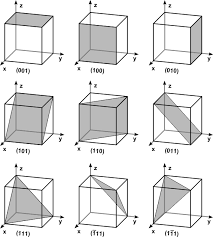
\includegraphics[width=0.5\linewidth]{miller}
\caption{Płaszczyzny zapisane w postaci wskaźników Millera.}
\label{fig:miller}
\end{figure}
Jesli płaszczyzna przecina osie $\vec{a}_1,\:\vec{a}_2,\:\vec{a}_3$ sieci w punktach o współrzednych odpowiednio $n_1,\: n_2,\: n_3$, to jej wskaźniki Millera to $\left(\frac{\alpha}{n_1},\frac{\alpha}{n_2},\frac{\alpha}{n_3}\right)$, gdzie $\alpha$ jest najmniejsza liczba dla której wskazniki sa liczbami
całkowitymi. Gdy płaszczyzna jest równoległa do którejs z osi, to odpowiedni wskaznik
wynosi $0$. Gdy którys ze wskazników jest ujemny, oznacza sie to nastepujaco: $(0\bar{1}0)$.
\subsection{Dyfrakcyjne metody badania kryształów}

pisac
Ponieważ odległości w kryształach są bardzo małe - rzędu $10^{-10}\:\mathrm{m}$, to nie możemy używać światła widzialnego do badań nad nimi. Musimy wykorzystać fale o długości porównywalnej do stałej sieci kryształu. Kryształy możemy badać poprzez dyfrakcję promieniowania elektormagnetycznego o odpowiednio krótkiej długości fali lub za pomocą fal materii(neutrony lub elektrony). Sieć krystaliczna zastępuje nam siatkę dyfrakcyjną.\\
Do opisu dyfrakcji możemy użyć Prawa Bragga:
\begin{align*}
2d\sin\theta=n\lambda
\end{align*}
Gdzie $d$ to odległość między płaszczyznami w krysztale, $\theta$ to kąt obserwacji a $\lambda$ to długość fali promieniowania.
\subsubsection{Metoda Lauego}
Metoda Lauego polega na oświetlaniu widmem ciągłym lampy rentgenowskiej spoczywajacego nieruchomo kryształu. Promienie ugięte rejestrowane są na kliszy
fotograficznej znajdujacej sie za kryształem (promienie przechodzące) lub przed kryształem (promienie zwrotne) – wtedy wiązka padająca przechodzi przez otwór wycięty w kliszy. Obrazy otrzymane na kliszach nazywa się lauegramami. Każda plamka na lauegramie odpowiada wiązce promieni odgiętych dla pewnej rodziny płaszczyzn oddalonych o $d$ dla pewnego kata $\theta$. Okazuje się, że plamki grupuję się wzdłuż krzywych
stożkowych (elips, parabol i nielicznych hiperbol dla metody promieni przechodzących, wyłącznie hiperbol dla promieni zwrotnych). Krzywe te są przecięciami płaszczyzn klisz ze stożkami interferencyjnymi wiązek ugiętych przez daną rodzinę płaszczyzn krystalograficznych. Metoda Lauego stosowana jest do badania orientacji kryształu, a także do badania
jego defektów, gdyż w przypadku wygięcia lub skręcenia próbki, plamki na lauegramach
ulegaja skręceniu i rozmyciu.
\subsubsection{Metoda proszkowa}
W metodzie proszkowej nie naświetla się monokryształu, lecz próbkę sproszkowana, umieszczona w kapilarze. Używa się również światła monochromatycznego, a nie ciągłego. Ponieważ – jak można przyjąć – w próbce kryształy występują w dowolnej orientacji, to naświetlenie jej jedna wiązka da obrazy ugięć na wszystkich płaszczyznach
krystalicznych. Ponadto wiązki ugięte tworzyć będą pełne stożki o kacie rozwarcia $4\theta$, ponieważ płaszczyzny nachylone do wiązki padające o $\theta$ (dające ugięcia o $2\theta$) mogą być dowolnie obrócone wokół osi. Cała próbkę otacza się paskiem kliszy fotograficznej tak, że obrazami są łuki elips. Metoda proszkowa stosowana jest często w metalurgii i innych dziedzinach, które nie dysponują dużymi monokryształami, tylko pyłem materiału.
\subsubsection{Metoda obracającego się kryształu}
Metoda obracanego kryształu polega na, jak sama nazwa wskazuje, naświetlaniu światłem monochromatycznym kryształu, który obracany jest wokół wybranej osi krystalograficznej. Kryształ otacza się klisza fotograficzna o kształcie walca, którego osia jest os obrotu kryształu. Po rozwinięciu błony otrzymuje się dyfraktogram, na którym ślady wiązek układają się w linie poziome – w tym przypadku taki własnie kształt
ma przecięcie stożków interferencji z klisza. Wadą tej metody jest fakt, ze wskutek ograniczeń obrotu kryształu do jednej osi pewne płaszczyzny nie dadzą refleksów, np. płaszczyzna prostopadła do osi obrotu. W naszym doświadczeniu zastosujemy pewna modyfikacje metody obracanego kryształu. Zamiast kliszy fotograficznej, która pozwala jedynie jakościowo opisać procesy dyfrakcyjne, promienie rentgenowskie będą mierzone licznikiem Geigera. Aby zapewnić
właściwe ustawienie licznika względem kryształu w czasie obrotów, zostanie on zamocowany na goniometrze, który pozwoli zsynchronizować obrót próbki (w centrum) i licznika (na ramieniu urządzenia) z odpowiednia $(2:1)$ proporcja prędkości kątowych. Kryształ będzie oświetlany światłem lampy rentgenowskiej, stąd w wynikowym wykresie dobrze będą widoczne ugięcia fal widma charakterystycznego. Przyjrzyjmy się sposobowi, w jaki zachodzi odbicie w metodzie obracanego kryształu. Załóżmy, że kryształ regularny obraca się wokół osi $[001]$. Ponieważ obrót sieci prostej jest jednocześnie obrotem sieci odwrotnej, siec odwrotna obraca się wokół wektora ~b3. Płaszczyzny $(hkl)$ kryształu są przedstawione w sieci odwrotnej przez punkty leżące w pierwszej warstwicy prostopadłej do $\vec{b}_3$. Obroty sieci odwrotnej powodują, ze płaszczyzna ta odcina na sferze odbicia koło. Oznacza to, że wektory wiązek ugiętych będą kończyć się na tym kole, zatem promienie ugięte będą leżeć na powierzchni stożka.
\begin{figure}[h!]
\centering
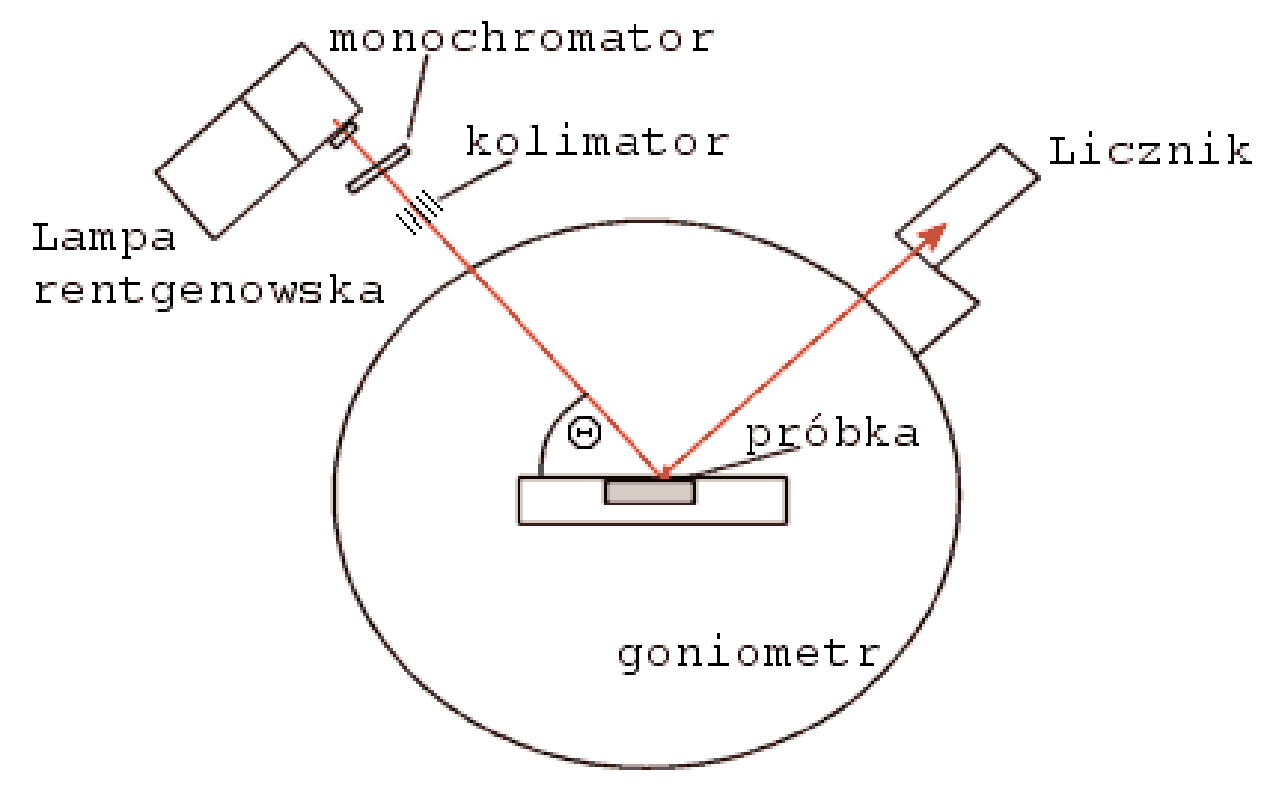
\includegraphics[width=0.8\linewidth]{obr}
\caption{Schemat układu pomiarowego.}
\label{fig:obr}
\end{figure}

\newpage
\section{Obliczenia}
\subsection{Wyznaczanie stałej Plancka}
Stałą Plancka wyznaczamy poprzez badanie krótkofalowej granicy falowej. Ta długość fali odpowiada sytuacji, gdy elektron oddaje całą swoją energię w postaci fotonu.
\begin{align*}
eU=h\nu=\frac{hc}{\lambda}\qquad\Rightarrow\qquad \lambda= \frac{hc}{eU}
\end{align*}
Dalej możemy skorzystać z Prawa Bragga dla dyfrakcji:
\begin{align*}
2d\sin\theta=n\lambda
\end{align*}
Czyli możemy wyrazić $\sin\theta$ jako:
\begin{align*}
\sin\theta=\frac{nhc}{2de}\frac{1}{U}
\end{align*}
Analizując wykresy natężenia promieniowania zależngo od kąta ustawienia kryształu, możemy zauważyć miejsce zanikania promieniowania. Jest to krótkofalowa granica promieniowania. Jednak w wyniku szumów, których nie da się wyeliminować eksperymentalnie, nie możemy odczytać wartości bezpośrednio z wykresu. W tym celu przybliżamy prostą odcinek krzywej, gdzie obserwujemy zanik promieniowania. Mają postać dopasowanej prostej, możemy wyznaczyć jej miejsce zerowe czyli kąt odpowiadający krótkofalowej granicy promieniowania.
\begin{figure}[h!]
\centering
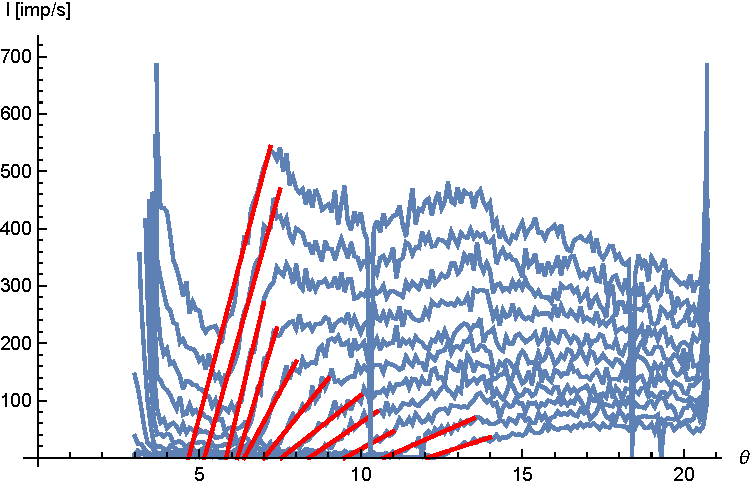
\includegraphics[width=0.75\linewidth]{allfits}
\caption{Dane dla różnych napięć przyspiesząjących z pomiarów dyfrakcji promieni X na krysztale LiF wraz z dopasowanymi prostymi umożliwiającymi ustalenie krótkofalowej granicy falowej.}
\label{fig:allfits}
\end{figure}\\
Możemy wykreślić zależność $\sin\theta$ od $\frac{1}{U}$ na podstawie danych z różnych pomiarów. Metodą najmniejszych kwadratów możemy znaleźć wartość współczynnika dla liniowej zależności $\sin\theta=\alpha \frac{1}{U}$. Zgodnie z pakietem zwartym w programie Mathematica wartość współczynnika wynosi $\alpha=3.09\pm0.023$.

Zgodnie z wyprowadzoną przez nas wcześniej zależnością możemy zapisać:
\begin{align*}
\alpha=\frac{nhc}{2de}\qquad\Rightarrow\qquad h=\frac{2\alpha d e}{nc}
\end{align*}
Skad możemy dostać wartość stałej Plancka:
\begin{align*}
h=6.65033\cdot10^{-34}
\end{align*}\\\begin{figure}[h!]
	\centering
	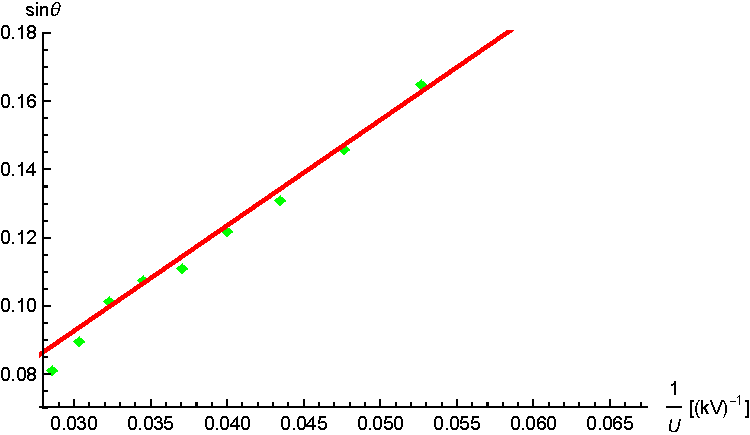
\includegraphics[width=0.9\linewidth]{fitsin}
	\caption{Zależność kąta odpowiadającego granicy krótkofalowej od odwrotności napięcia.}
	\label{fig:fitsin}
\end{figure}\\
Korzystaliśmy z następujących wartości wielkości fizycznych[3]:
\begin{itemize}
	\item prędkość światła: $c=299792458\:\mathrm{\frac{m}{s}}$
	\item ładunek elementarny: $e=1.60217662\cdot 10^{-19}\:\mathrm{C}$
	\item odległość między kolejnymi płaszczyznami dyfrakcyjnymi, będąca połową długości, ze względu na dwuatomową bazę, stałej sieci dla płaszczyzny $(100)$: $d=201.4\:\mathrm{pm}$
	\item rząd dyfrakcji: $n=1$
\end{itemize}
\newpage
 \subsection{Stała sieci krystalicznej}
 Przeprowadziliśmy pomiar dyfrakcyjny dla kryształu NaCl przy prądzie $I=1\:\mathrm{mA}$ i napięciu $U=35\:\mathrm{kV}$. Na wykresach możemy zidentyfikować odpowiednie maksima dyfrakcyjne.
 \begin{figure}[h!]
\centering
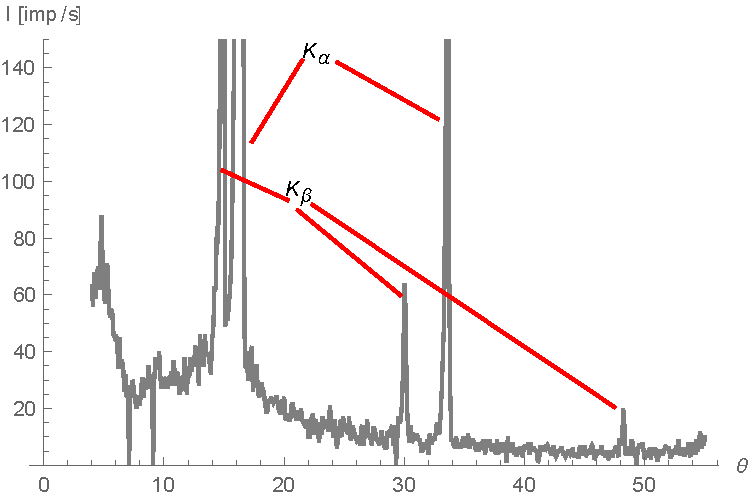
\includegraphics[width=0.8\linewidth]{nacl}
\caption{Pomiar dyfrakcyjny dla próbki NaCl}
\label{fig:nacl}
\end{figure}\\
Dokładne wartości dla maksimów:
\begin{table}[h!]
	\begin{tabular}{|l|l|l|l|l|l|}
		\hline
		Linia charakterystyczna & $\alpha$ & $\alpha$ & $\beta$ & $\beta$ & $\beta$ \\ \hline
		Rząd dyfrakcji          & 1    & 2    & 1    & 2    & 3    \\ \hline
		Kąt $[\:^\circ]$ & 16.5 & 33.6 & 14.9 & 30.0 & 48.2 \\ \hline
	\end{tabular}
\end{table}\\
Teraz możemy skorzystać z wyrażenia dyfrakcji Bragga(uwzględniamy, że w krysztale NaCl stała sieci równa się podwojonej odległości międzypłaszczyznowej):
\begin{align*}
2\frac{d}{2}\sin\theta=n\lambda\qquad\Rightarrow\qquad d=\frac{n\lambda}{\sin\theta}
\end{align*}

Długości fali dla poszczególnych linii charakterystycznych to $\lambda_\alpha=154.05\:\mathrm{pm}$ i $\lambda_\beta=139.23\:\mathrm{pm}$.
\begin{table}[h]
	\begin{tabular}{|l|l|l|l|l|l|}
		\hline
		Stała sieci $[\mathrm{m}]$ & $5.424\cdot10^{-10}$ & $5.56749\cdot10^{-10}$ & $5.41471\cdot10^{-10}$ & $5.5692\cdot10^{-10}$ & $5.603\cdot10^{-10}$ \\ \hline
	\end{tabular}
\end{table}\\
Wartość średnia z tych wartości to:
\begin{align*}
d=5.51568\cdot10^{-10}\:\mathrm{m}=5.51568\:\mathrm{\AA}
\end{align*}
\section{Niepewność pomiarowa}
\subsection{Stała Plancka}
Prawo przenoszenia niepewności dla pomiaru stałej Plancka:
\begin{align*}
u(h)=\sqrt{\left(\frac{\partial h}{\partial \alpha}u(\alpha)\right)^2}=\frac{2d e}{nc}u(\alpha)
\end{align*}
Dla $d(\alpha)=0.023$ oraz wymienionych wcześniej wielkości:
\begin{align*}
u(h)=4.95116\cdot 10^{-36}\approx0.049\cdot 10^{-34}
\end{align*}
\subsection{Stała sieci}
By obliczyć niepewność naszych pomiarów zastosujemy niepewność standardową, która jest postaci:
\begin{align}
u(a)=\sqrt{\frac{1}{n(n-1)}\sum\limits_{i=1}^{n}\left(a_i-\bar{a}\right)^2}
\end{align}
W naszym przypadku niepewność stałej sieci:
\begin{align*}
u(d)=3.98572\cdot10^{-12}\approx 4\cdot10^{-12}\:\mathrm{m}=0.04\:\mathrm{\AA}
\end{align*}
\section{Wnioski}
\subsection{Stała Plancka}
Tablicowa wartość stałej Plancka to: $h=6.63\cdot 10^{-34}\:\mathrm{J\cdot s}$ [3].\\
Nasz wynik, to $h=(6.65\pm0.049)\cdot 10^{-34}\:\mathrm{J\cdot s}$. \\Różni się on o $0.3\%$ od wartości tablicowej, co jest bardzo dobrym wynikiem. A wartość tablicowa mieści się w przedziale niepewności.

Jak widać jest to bardzo dokładna metoda wyznaczania stałej Plancka.
\subsection{Stała sieci}
Tablicowa wartość stałej sieci NaCl: $d=5.641\:\mathrm{\AA}$.\\
Nasz wynik to $d=(5.52\pm0.04)\:\mathrm{\AA}$. Wartość tabelaryczna nie mieści się w przedziale niepewności. Różnica od wartości tabelarycznej to ponad $2\%$. Nie jest to wynik nieprawdziwy, wciąż jesteśmy blisko wartości rzeczywistej, jednak możnaby się zastanowić jak poprawić nasze pomiary.\\
Nie mieliśmy istotnego wpływu na proces pomiaru, nie licząc drobnych rożnic przy konfiguracji układu, które nie mogły mieć istotnego wpływu na jego wynik. Proces analizy danych również nie niósł za sobą możliwwości błędnych założeń analizatora. 
Możliwe, że seria pomiarów dałaby możliwość wyelimiowania szumu pomiarowego i lepszych wyników.
\newpage
\begin{thebibliography}{99}
	\bibitem{1} Ch. Kittel, \textit{Wstęp do fizyki ciała stałego}, PWN, Warszawa 1999.
	\bibitem{2} Sz. Szczeniowski, \textit{Fizyka doświadczalna}, t.5 PWN, Warszawa
	1974.
	\bibitem{dyf}
	Bernard Dennis Cullity, \emph{Podstawy dyfrakcji promieni rentgenowskich}, PWN, Warszawa
	1964.
	\bibitem{boj}
	Zbigniew Bojarski, Eugeniusz Łagiewka, \emph{Rentgenowska analiza strukturalna}, PWN,
	Warszawa 1988.
	\bibitem{3}
	T. Szymczyk, \emph{Tablice matematyczne, fizyczne, astronomiczne i chemiczne}, PPU "PARK", Bielsko-Biała 2002.
\end{thebibliography}
\end{document}